\documentclass{sig-alternate}
\usepackage{algorithm,algpseudocode}
\usepackage{url}

\begin{document}

\conferenceinfo{HPDC}{'12 Delft, The Netherlands}
% \CopyrightYear{2007} % Allows default copyright year (20XX) to be over-ridden
% - IF NEED BE. \crdata{0-12345-67-8/90/01}  % Allows default copyright data
% (0-89791-88-6/97/05) to be over-ridden - IF NEED BE.

\title{Cost- and Deadline-constrained Scheduling of Scientific Workflow Ensembles in IaaS Clouds}
% \subtitle{[Extended Abstract]}

\numberofauthors{2}
\author{
    \alignauthor Maciej Malawski and Jarek Nabrzyski\\
       \affaddr{University of Notre Dame}\\
       \affaddr{Center for Research Computing}\\
       \affaddr{111 Information Technology Center}\\
       \affaddr{Notre Dame, IN, USA}\\
       \email{\{mmalawsk,naber\}@nd.edu}
    \alignauthor Gideon Juve and Ewa Deelman\\
       \affaddr{USC Information Sciences Institute}\\
       \affaddr{4676 Admiralty Way}\\
       \affaddr{Marina del Rey, CA, USA}\\
       \email{\{gideon,deelman\}@isi.edu}
}

\maketitle
 
\begin{abstract}
Abstract goes here.
\end{abstract}

%\category{H.4}{Information Systems Applications}{Miscellaneous}
%\category{D.2.8}{Software Engineering}{Metrics}[complexity measures, performance measures]

%\terms{Theory}

\keywords{Scientific workflows, DAG scheduling, simulation}

\section{Introduction}

Scientific workflows, usually represented as directed acyclic graphs (DAG), are
the important class of applications that have been studied in the context of
resource management and scheduling on grid and utility computing systems.
However, large computational applications are often composed of several 
inter-related workflows grouped into {\em ensembles}. All the
workflows in an ensemble typically have a similar structure, but they differ by
input data, number of tasks and individual tasks sizes. A good example of
scientific workflow ensemble comes from the CyberShake
application~\cite{Callaghan11}, which calculates seismic hazards for a given
geographical region such as California. In order to produce a hazard map, the
hazard curves need to be computed for a set of geographical sites, while each
site requires running a single complex scientific workflow. Workflows for each
site may differ not only by their parameters, but also by priority; e.g. some of
the points on the map correspond to urban areas or strategic locations such as
power plants, whereas others may be located in less populated regions. Another
example of workflow ensembles comes from astronomical applications, such as
Montage~\cite{Deelman08} or search for Earth-like planets from Kepler project
data~\cite{vockler11}, where multiple, different workflows are used to
process data for different areas of the sky.

Infrastructure-as-a-Service (IaaS) clouds offer the ability to provision 
computational resources on-demand according to a pay-per-use model. These systems 
are regarded by the scientific community as a potentially attractive source of 
low-cost, on-demand computing resources~\cite{Ostermann10,Keahey09}. In contrast 
to clusters and grids, which typically offer best-effort quality of service, clouds 
give users more flexibility to creating a controlled and managed computing environment
with the ability to adjust resource capacity according to the dynamically changing
computing demands of the application, often called auto-scaling. Giving the users 
more control, however, also requires the development of new methods for task 
scheduling and resource provisioning. The resource management decisions required 
in cloud scenarios not only have to take into account traditional performance-related 
metrics such as workflow makespan or resource utilization, but must also now consider
budget constraints, since the resources from public (commercial) cloud providers 
are usually not free~\cite{Durkee10}.

In this paper, to get insight into these resource management challenges for
scientific workflows on clouds, we address a new important problem of maximizing
the number of completed workflows from an ensemble under both budget and
deadline constraints. The motivation is to answer the fundamental question of a
researcher: How much computation can be completed given the limited budget and 
timeframe of a research project? The goals of this paper are to discuss and assess possible
static and dynamic strategies for both task scheduling and resource
provisioning. Based on the knowledge of workflow scheduling algorithms we
analyze strategies for on-line scheduling of individual tasks as well as static
algorithms that rely on the information about the workflow structure (critical
paths and workflow levels) and estimates of task runtimes. In addition, we
analyze a hybrid workflow-aware dynamic scheduling algorithm, which uses the
workflow structure information to estimate which workflows should be rejected
from the ensemble due to the constraints. As methodology in the study of the
proposed algorithms we use simulation techniques. We have developed cloud workflow simulator based on
CloudSim~\cite{Calheiros11}, which models the infrastructure and the application. The
algorithms are subject to evaluation on a set of scientific workflow ensembles with a broad range of
budget and deadline parameters. 

The paper is organized as follows [\ldots]

\section{Related Work}
General policy and rule-based approaches to dynamic provisioning (e.g. Amazon
Auto Scaling\footnote{\url{http://aws.amazon.com/autoscaling}} and
RightScale\footnote{\url{http://www.rightscale.com}}) allow adjusting the size
of resource pool based on metrics related to infrastructure and application.
Typical infrastructure-specific metric is system load, whereas
application-specific metrics include response time and queue length. It is
possible to set thresholds and limits to tune the behavior of these autoscaling
systems, but no support for complex applications is provided.

Policy-based approaches for scientific workloads (e.g. \cite{Marshall2010,
Kim2011}) also allow to scale the the cloud resource pool or to extend the
capabilities of clusters using cloud-burst techniqies. Our approach is different
in that we consider workflows, while policy based approaches typically consider
bags of independent tasks or unpredictable batch workloads. This enables us to
take advantage of scheduling heuristics that cannot be applied to independent
tasks.


Our work is related to the strategies for deadline-constrained cost-minimization
workflow scheduling, developed for utility grid systems. However, our problem is
different from \cite{Yu2005, Abrishami2010} in that we consider ensembles of workflows in
IaaS clouds, which allow one to provision resources on a per-hour billing model,
rather than utility grids, which allow one to choose from a pool of existing
resources with a per-job billing model. Our work is also different from
cloud-targeted autoscaling solution~\cite{Mao2011} in that we consider ensembles
of workflows rather than unpredictable workloads containing workflows. We also have budget constraints
rather than cost minimization as a goal. In other words, we assume that there is
more work to be done than the available budget, so some work must be rejected.
Therefore cost is not something we optimize, but rather a constraint.


We should refer to bi-criteria scheduling and multi-criteria scheduling of
workflows~\cite{Wieczorek2009,Prodan10,Dongarra2007}. These approaches are
similar to ours in that we have two scheduling criteria: cost and makespan. The
challenge in multi-criteria scheduling is to derive an objective function that
takes into account all of the criteria. In our case one objective (amount
of work completed) is subject to optimization, whereas time and cost are
trated as constraints. Other approaches~\cite{Talukder2009,Pandey2010} use
metaheuristics that usually run for a long time before producing good results,
which makes tham less useful in practical applications. Our work can be also
regarded as extension of the budget-constrained workflow scheduling
\cite{Sakellariou2007} in the sense that we are dealing with workflow ensembles
and the deadline constraint is added.
 
\section{Problem Description}
\subsection{Resource Model}
Describe the Amazon EC2 resource model. Instances are requested on-demand. Instance pricing is per-hour. Multiple VM types are available, but for this paper we focus on a single VM type because we assume that there will typically be one VM type with the best price/performance ratio for the application.

\subsection{Application Model}
The target applications for this paper are scientific workflows that can be modeled as Directed Acyclic Graphs (DAGs).

We assume that we have runtime estimates for each task in the workflow.

Currently we do not consider data sizes, but rather assume that data is stored in a shared cloud storage system such as Amazon S3 and that data transfer times are included in task runtime estimates. Further, data transfer times are equal across the VMs.

An ensemble consists of several related workflows. Each workflow is given a priority.

The goal is to complete as many workflows as possible given a budget and a deadline.


\section{Algorithms}

In this section we describe several algorithms we developed to execute ensembles of
workflows on the cloud under budget and deadline constraints.

\subsection{Static Provisioning Dynamic Scheduling \\
(SPDS) }
\label{sec:spds}

The simplest strategy for executing ensembles of workflows in the cloud is to
provision resources statically and schedule workflow tasks dynamically. Given a 
budget $b$, deadline $d$, and the hourly price $p$ of a VM, it is easy to calculate
the number of VMs, $N_{VM}$, to provision so that the entire budget is consumed before
the deadline:

\begin{equation}
\label{eq:static-plan}
N_{VM} = \lceil b / d / p \rceil
\end{equation}

The SPDS algorithm statically provisions $N_{VM}$ VMs at the start of the ensemble execution 
and keeps them running until the deadline is reached, or the budget runs out.
This provisioning plan has the advantage that it minimizes the number of provisioning 
and de-provisioning requests.

Once the VMs are provisioned, the tasks are mapped onto idle VMs using the dynamic
priority-based scheduling procedure shown in Algorithm~\ref{alg:ds}.

\begin{algorithm}
\caption{Priority-based scheduling algorithm for SPDS}
\label{alg:ds}
\begin{algorithmic}[1]
\Procedure{Schedule}{}
    \State $P\gets$ empty priority queue
	\State $IdleVMs\gets$ set of idle VMs
	\For{root task $t$ in all workflows}
    	\State \Call{Insert}{$t,P$} 
    \EndFor
    \While{deadline not reached}
    	\While{$IdleVMs \neq \emptyset\ and\ P \neq \emptyset$}
    		\State $v\gets$ \Call{SelectRandom}{$IdleVMs$}
    		\State $t\gets$ \Call{Pop}{$P$}
    		\State \Call{Submit}{$t,v$}
    	\EndWhile
    	\State Wait for task $t$ to finish on VM $v$
    	\State Update $P$ with ready children of $t$
		\State \Call{Insert}{$v,IdleVMs$}
    \EndWhile
\EndProcedure
\end{algorithmic} 
\end{algorithm}

Initially, the ready tasks from all workflows in the ensemble are added to a 
priority queue based on the priority of the workflow to which they belong. If
there are idle VMs available, and the priority queue is not empty, the next task
from the priority queue is submitted to a randomly chosen idle VM. The process is 
repeated until there are no idle VMs or the priority queue is empty. The scheduler
then waits for a task to finish, adds its ready children to the priority queue,
marks the VM as idle, and the entire process repeats until the deadline is reached.

This algorithm guarantees that tasks from lower priority workflows are
always deferred when higher-priority tasks are available, but lower-priority
tasks can still occupy idle VMs when higher-priority tasks are not available. 
However, because there is no preemption, long-running low-priority tasks may delay 
the execution of higher-priority tasks. In addition, tasks from low priority 
workflows may be executed even though there is no chance that those workflows 
will be completed within the current budget and deadline. Fig.~\ref{fig:spds-example} 
shows an example schedule generated using the SPDS algorithm. The figure illustrates 
how tasks from lower priority workflows backfill idle VMs when tasks from higher 
priority workflows are not available.

\begin{figure}[htb] 
\centering
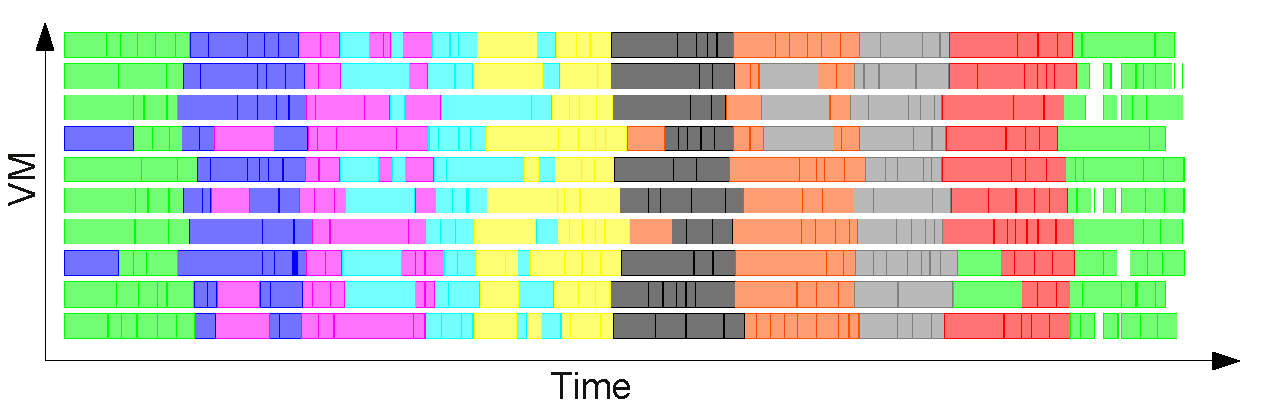
\includegraphics[width=1.0\columnwidth]{figures/spds-gantt}
 \caption{Example schedule generated using SPDS algorithm. Tasks are colored by workflow. }
\label{fig:spds-example}
\end{figure}

\subsection{Dynamic Provisioning Dynamic \\Scheduling (DPDS)}
 
The static provisioning approach of SPDS may not be optimal when resource demand
changes during ensemble execution. In those cases, SPDS may either over-provision, 
wasting the budget on idle VMs, or under-provision, using up the deadline while starving 
the application of usable VMs. One of the advantages of elasticity in cloud computing 
is that the number of resources can be changed to meet the demands of an application.
In policy-based provisioning (or auto-scaling) systems, metrics such as resource 
utilization and queue length are monitored to estimate application demand. The DPDS 
algorithm uses this approach to determine when to provision and de-provision VMs. The 
algorithm periodically computes resource utilization as the percentage of idle VMs, and
adjusts the number of VMs if the utilization is above or below given thresholds.
Because it is assumed that VMs are billed by the hour, DPDS only considers VMs that are
approaching their hourly billing cycle when deciding which VMs to terminate. This process
is described in Algorithm~\ref{alg:prov}.

\begin{algorithm}
\caption{Dynamic provisioning algorithm for DPDS}
\label{alg:prov}
\begin{algorithmic}[1]
\Require $c$: consumed budget; $b$: total budget; $d$: deadline; $p$: price;
$t$: current time; $u_h$: upper utilization threshold; $u_l$: lower utilization
threshold; $v_{max}$: maximum number of VMs
\Procedure{Provision}{}
	\State $V_R\gets$ set of running VMs
    \State $V_C\gets$ set of VMs completing billing cycle
    \If{$ b - c < |V_C| * p\ or\ t > d $ }
    	\State $n_T\gets |V_R| - \lfloor(b-c)/p\rfloor$
    	\State $V_T\gets$ select $n_T$ VMs to terminate from $V_C$
    	\State \Call{Terminate}{$V_T$} \label{l:terminate1}
    \Else 
		\State $u\gets$ current VM utilization
    	\If{$u>u_h$ and $|V_R| < v_{max}*N_{VM}$}
    		\State \Call{Start}{$new\ VM$}
    	\ElsIf{$u<u_l$}
    		\State $V_I\gets$ set of idle VMs
    		\State $n_T\gets \lceil|V_I|/2\rceil$ \label{l:nT2}
			\State $V_T\gets$ select $n_T$ VMs to terminate from $V_I$
    		\State \Call{Terminate}{$V_T$} \label{l:terminate2}
    	\EndIf 
    \EndIf
\EndProcedure
\end{algorithmic} 
\end{algorithm}

The set of VMs completing their billing cycle is determined by considering both the
provisioner interval, and the termination delay of the provider. This guarantees 
that VMs can be terminated before they start the next billing cycle and prevents the
budget from being overrun. The VMs terminated in line \ref{l:terminate1} are the ones 
that would overrun the budget if not terminated in the current provisioning cycle. 
The VMs terminated on line \ref{l:nT2} are chosen to increase the resource utilization
to the desired threshold. In order to prevent instances from being
terminated too quickly, potentially wasting resources that have already been paid for
but could be used later, no more than half of the idle resources are terminated during
each provisioning cycle. To avoid an uncontrolled increase in the number of
instances, which may happen in the case of highly parallel workflows, the provisioner 
will not start a new VM if the number of running VMs is greater than the product of
$N_{VM}$ and an autoscaling factor, $v_{max}$.


\subsection{Workflow-Aware DPDS (WA-DPDS)}

The DPDS algorithm does not use any information about the structure of the workflows
in the ensemble when scheduling tasks: it looks only at the priorities of the ready 
tasks when deciding which task to schedule next. It does not consider whether a lower 
priority task belongs to a workflow that it will never be able to complete given the 
current budget and deadline. As a result, DPDS may execute lower priority tasks just 
to keep VMs busy that will end up delaying higher priority tasks, making it less likely
that higher priority workflows will be able to finish.

In order to address this issue, the Workflow-Aware DPDS (WA-DPDS) algorithm extends 
DPDS by introducing a workflow admission procedure. The admission procedure is
invoked whenever WA-DPDS sees the first task of a new workflow at the head of the 
priority queue (i.e. when no other tasks from the workflow have been scheduled yet). 
The admission procedure---shown in Algorithm~\ref{alg:wa-dpds}---estimates if there is 
enough budget remaining to admit the new workflow; if there is not, then the 
workflow is rejected and its tasks are removed from the queue. This algorithm 
compares the current cost (consumed budget) and remaining budget, taking
into account the cost of currently running VMs, and the cost of workflows 
that have already been admitted. It adds a small safety margin avoid going over
the budget.

\begin{algorithm}
\caption{Workflow admission algorithm for WA-DPDS}
\label{alg:wa-dpds}
\begin{algorithmic}[1]
\Require $w$: workflow; $b$: budget; $c$: current cost
\Procedure{Admit}{$w,b,c$}
    \State $r_n\gets b-c$ \Comment{Budget remaining for new VMs}
    \State $r_c\gets $cost committed to VMs that are running
    \State $r_a\gets $cost to complete workflows previously admitted
	\State $r_m\gets 0.1$ \Comment{Safety margin}
	\State $r_b\gets r_n+r_c-r_a-r_m$ \Comment{Budget remaining}
	\State $c_w\gets$ \Call{EstimateCost}{w}
    \If{$c_w<r_b$}
    	\State \textbf{return} $TRUE$
    \Else
    	\State \textbf{return} $FALSE$
	\EndIf    	 
\EndProcedure
\end{algorithmic} 
\end{algorithm}


This admission procedure relies only on the total estimated resource consumption and
compares it to the budget remaining. We found that this estimation is useful not
only to prevent low-priority workflows from delaying high-priority ones, but
also to reject large and costly workflows that would overrun the budget and
admit smaller workflows that can efficiently utilize idle resources in ensembles 
containing workflows of non-uniform sizes. It would also be possible to extend this 
admission procedure to check other constraints, such as whether the estimated 
critical path of the new workflow exceeds the time remaining until the deadline.



\subsection{Static Provisioning Static Scheduling \\(SPSS)}

The previous algorithms are all online algorithms that make provisioning 
and scheduling decisions at runtime. In comparison, the SPSS algorithm 
creates a provisioning and scheduling plan before running any workflow tasks.
This enables SPSS to start only those workflows that it knows can be completed
given the deadline and budget constraints, and eliminates any waste that may
be allowed by the dynamic algorithms.

The approach used by SPSS is to plan each workflow in the ensemble in priority 
order, rejecting any workflows that cannot be completed by the deadline or that 
cause the cost of the plan to exceed the budget. Once the plan is complete, then 
the VMs are provisioned and tasks are executed according to the schedules given
by the plan.

The disadvantage of the static planning approach used by SPSS is that it is 
sensitive to dynamic changes in the environment and the application that may 
disrupt the carefully constructed plan.

Algorithm~\ref{alg:admit} shows how ensembles are planned in SPSS. The algorithm
starts with an empty plan containing no VMs and no scheduled tasks. Workflows
from the ensemble are considered in priority order. For each workflow, SPSS
attempts to build on top of the current plan by provisioning VMs to schedule 
the tasks of the workflow so that it finishes before the deadline with the least
possible cost. If the cost of the new plan is less than the budget, then the 
new plan is accepted and the workflow is admitted. If not, then the new plan is 
rejected and the process continues with the next workflow in the ensemble. The 
idea behind this algorithm is that, if each workflow can be completed by the 
deadline with the lowest possible cost, then the number of workflows that can 
be completed within the given budget will be maximized.

\begin{algorithm}
\caption{Ensemble planning algorithm for SPSS}
\label{alg:admit}
\begin{algorithmic}[1]
\Require $W$: workflow ensemble; $b$: budget; $d$: deadline
\Ensure Schedule as much of $W$ as possible given $b$ and $d$
\Procedure{PlanEnsemble}{$W,b,d$}
    \State $P\gets \emptyset$ \Comment{Current plan}
    \State $A\gets \emptyset$ \Comment{Set of admitted DAGs}
    \For{$w\ in\ W$}
        \State $P^\prime \gets$\ \Call{PlanWorkflow}{$w,P,d$}
        \If{$Cost(P^\prime) \le b$}
            \State $P\gets\ P^\prime$ \Comment{Accept new plan}
            \State $A \gets A\ +\ w$ \Comment{Admit w}
        \EndIf
    \EndFor
    \State \textbf{return} $P,A$
\EndProcedure
\end{algorithmic}
\end{algorithm}

In order to plan a workflow, the SPSS algorithm assigns 
sub-deadlines to each individual task in the workflow, and then schedules 
each task so as to minimize the cost of the task while still meeting its 
assigned sub-deadline. The idea is that if each task can be completed by 
its deadline in the least expensive manner possible, then the cost of the
entire workflow can be minimized without exceeding the ensemble deadline.

SPSS assigns sub-deadlines to each task based on the \emph{float time}
of the workflow. The float time is the amount of extra time that a workflow
can extend its critical path and still be completed by the ensemble deadline.
For a workflow $w$, the float time of $w$ is:

$$
FT(w) = d - CP(w)
$$

where $d$ is the ensemble deadline and $CP(w)$ is the critical path of $w$.
We assume that $CP(w) \leq d$, otherwise the workflow cannot be completed 
by the deadline and must be rejected. For large ensembles we expect the 
critical path of any individual workflow to be much less than the deadline.

SPSS distributes the float time of the workflow by level, so that each level
of the workflow gets a portion of the workflow's float time proportional to
the number of tasks in the level and the total runtime of tasks in the level.
The idea is that levels containing many tasks and large runtimes should be given
a larger portion of the float time so that tasks in those levels may be serialized.
Otherwise, many resources need to be allocated to run all of the tasks in 
parallel, which may be more costly.

The float time of a level $l$ in workflow $w$ is given by:

$$
FT(l) = FT(w) \Biggl[\left({\alpha}\frac{N(l)}{N(w)}\right) + \left({(1 - \alpha)}\frac{R(l)}{R(w)} \right)\Biggr]
$$

where $N(w)$ is the number of tasks in the workflow, $N(l)$ is the number of tasks 
in level $l$, $R(w)$ is the total runtime of all tasks in the workflow, $R(w)$ is
the total runtime of all tasks in level $l$, and $\alpha$ is a parameter between
0 and 1 that causes more float time to be given to levels with more tasks (large 
$\alpha$) or more runtime (small $\alpha$). We set $\alpha$ to be 0.7.

The deadline of a task $t$ is then:

$$
DL(t) = LST(t) + RT(t) + FT(Level(t))
$$

where $Level(t)$ is the level of $t$, $RT(t)$ is the runtime of $t$, and $LST(t)$ 
is the latest start time of $t$ determined by:

$$
LST(t) = \begin{cases}
0,&$if t is a root task$\cr
\max_{p \in Pred(t)} DL(p),&$otherwise.$\cr
\end{cases}
$$

Algorithm~\ref{alg:planworkflow} shows how SPSS creates low-cost plans for
each workflow. The \textsc{PlanWorkflow} procedure first calls 
\textsc{DeadlineDistribution} to assign sub-deadlines to tasks according
to the procedure described above. Then, the \textsc{PlanWorkflow} procedure
schedules tasks onto VMs, allocating new VMs when necessary. For each task 
in the workflow, the the least expensive slot is chosen to schedule the 
task so that it can be completed by  its deadline. VMs are allocated in 
blocks of one billing cycle (one hour) regardless of the size of the task. 
When computing the cost of scheduling a task on a given VM, the algorithm 
considers idle slots in blocks that were allocated for previous tasks to be 
free, while slots in new blocks cost the full price of the new block. For 
example, if a task has a runtime of 10 minutes, and the price of a one-hour 
billing cycle is \$1, then the algorithm will either schedule the task on 
an existing VM that has an idle slot larger than 10 minutes for a cost of \$0, 
or it will allocate a new block on an existing VM, or provision a new VM, for 
a cost of \$1. If the cost of slots on two different VMs is equal, then the 
slot with the earliest start time is chosen. To prevent too many VMs from 
being provisioned, the algorithm always prefers to extend the runtime of 
existing VMs before allocating new VMs. The result of this is that the 
algorithm will only allocate a new block if there are no idle slots on 
existing blocks large enough or early enough to complete the 
task by its deadline, and it will only allocate a new VM if it cannot add 
a block to an existing VM to complete the task by its deadline.

\begin{algorithm}
\caption{Workflow planning algorithm for SPSS}
\label{alg:planworkflow}
\begin{algorithmic}[1]
\Require $w$: workflow; $P$: current plan; $d$: deadline
\Ensure Create plan for $w$ that minimizes cost and meets deadline $d$
\Procedure{PlanWorkflow}{$w,P,d$}
    \State $P^\prime\gets$ copy of $P$
    \State \Call{DeadlineDistribution}{w,d}
    \For{$t\ in\ w\ sorted\ by\ DL(t)$}
        \State $v \gets$ VM that minimizes cost and start time of t
        \If{$FinishTime(t,v) < DL(t)$}
            \State Schedule(t,v)
        \Else
            \State Provision a new VM v
            \State Schedule(t,v)
        \EndIf
    \EndFor
    \State \textbf{return} $P^\prime$
\EndProcedure
\end{algorithmic}
\end{algorithm}

An example schedule generated by SPSS is shown in Fig.~\ref{fig:spss-example}.
This example shows how SPSS tends to start many workflows in parallel, running
each workflow over a longer period of time on only a few VMs to minimize cost. 
In comparison, the dynamic algorithms tend to run one workflow at a time across 
many VMs in parallel.

\begin{figure}[htb] 
\centering
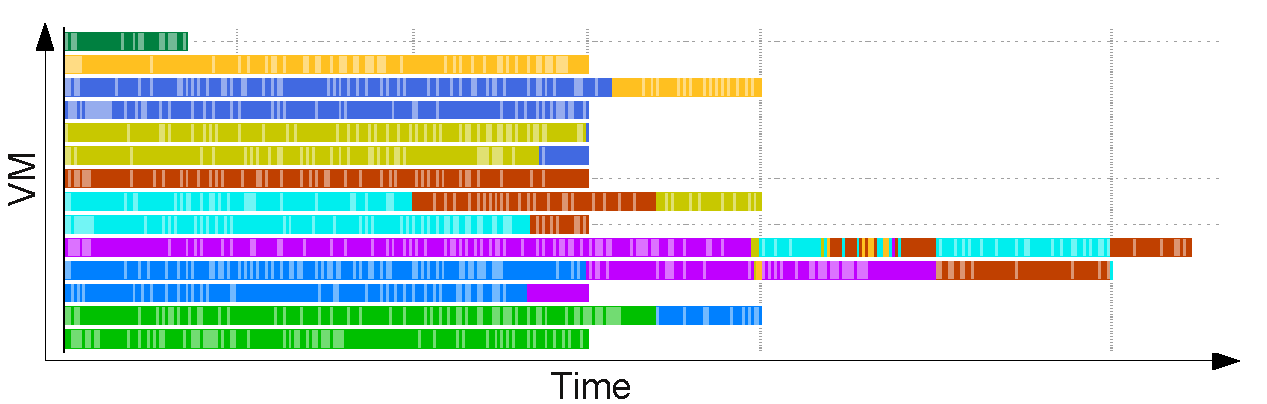
\includegraphics[width=1.0\columnwidth]{figures/spss-gantt}
 \caption{Example of schedule generated using SPSS algorithm. Tasks are colored by workflow. }
\label{fig:spss-example}
\end{figure}


\section{Performance Evaluation}

\subsection{Simulator}

To evaluate our algorithms, we developed a cloud workflows simulator based on
CloudSim~\cite{Calheiros11}. To represent our infrastructure model, we defined
Cloud, VM and WorkflowEngine simulation entities. Cloud object is responsible
for staring and terminating VMs using API similar to Amazon EC2. VM object is
responsible for execution of individual tasks, while WorkflowEngine deals with
management of ensembles and workflows. WorkflowEngine uses separate, although
tightly coupled Scheduler and Provisioner modules. We assume that a single core
of a VM executed submitted tasks sequentially and that a task is given exclusive
access to allocated VM. Although CloudSim provides a more advanced
infrastructure model which includes time-sharing and space-sharing policies and
power consumption in a datacenter, we do not use these features, since we are
interested mainly in execution of tasks on VMs and high-level workflow scheduling
on top of that. The simulator relies on DAG and DAX format used by Pegasus
project and workflow gallery.

\subsection{Scenarios}
\label{sec:scenarios}

We have prepared test scenarios to evaluate the proposed algorithms under
such a range of parameters that allows to observe the interesting properties of
algorithms for smaller and larger constraints. For a given ensemble we can
expect in general that the number of work done (in terms of workflows completed)
mainly depends on the budget constraint, which determines the number of
machine-hours that can be provisioned. The ideal but trivial case is then a
deadline long enough to allow running all the workflow tasks sequentially: this
eliminates all the overheads of parallel execution and leads to the highest
resource utilization. More interesting are the cases when the deadline is
shorter, since it forces provisioning of multiple VMs and thus increases
overheads due to parallel execution so the budget cannot be spent so
efficiently.

\begin{figure}[tb] 
\centering
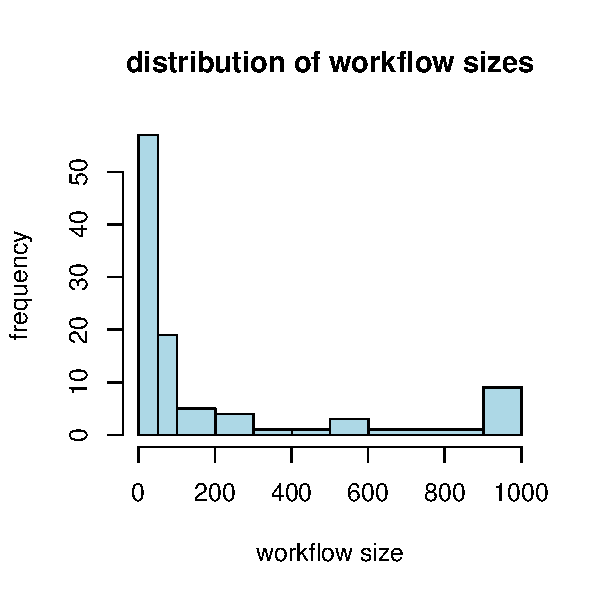
\includegraphics[width=0.6\columnwidth]{figures/ensemble-pareto}
\caption{Pareto-like distribution of workflow sizes in ensemble. Size is
measured in number of tasks.}
\label{fig:ensemble-distribution}
\end{figure}



We assumed that the interesting number of workflows in ensemble should be in the
order of between 10 and 100 workflows. This is motivated by several reasons:
first, such numbers are typical for the real applications, e.g. the number of geographical sites for
CyberShake workflow is in the order of 100. Second, the smaller ensembles
consisting of just a few workflows can be aggregated in a single workflow so
there is no need to treat them as ensembles. Similarly, when the number of
workflows is larger that 100 and each workflow has a large number of parallel
tasks, the problem of efficiently allocating them to the resources becomes much
easier and similar to the bag-of-tasks problem.


\begin{figure*}[t] 
\centering
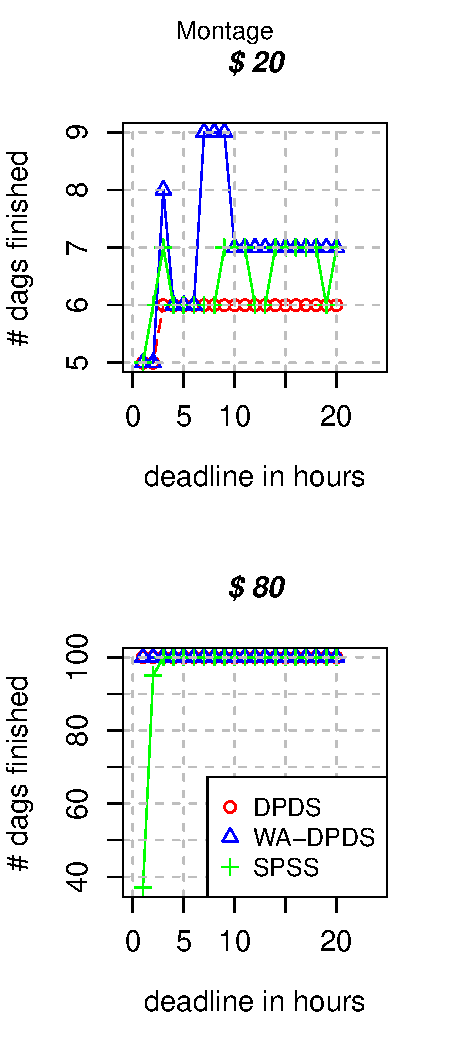
\includegraphics[width=0.19\textwidth]{figures/pareto-MONTAGE-n-1000-8-dagh1-20m0.pdf}
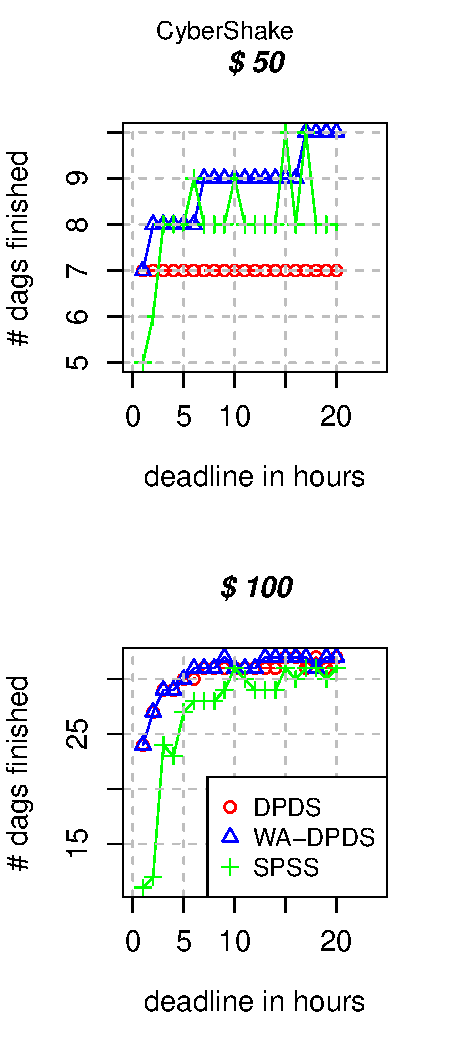
\includegraphics[width=0.19\textwidth]{figures/pareto-CYBERSHAKE-n-1000-8-dagh1-20m0.pdf}
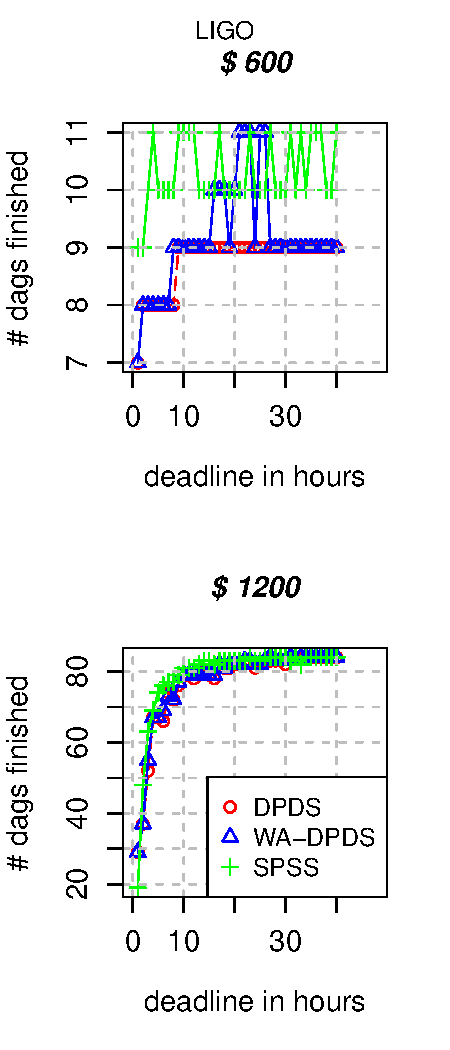
\includegraphics[width=0.19\textwidth]{figures/pareto-LIGO-n-1000-8-dagh1-40m0.pdf}
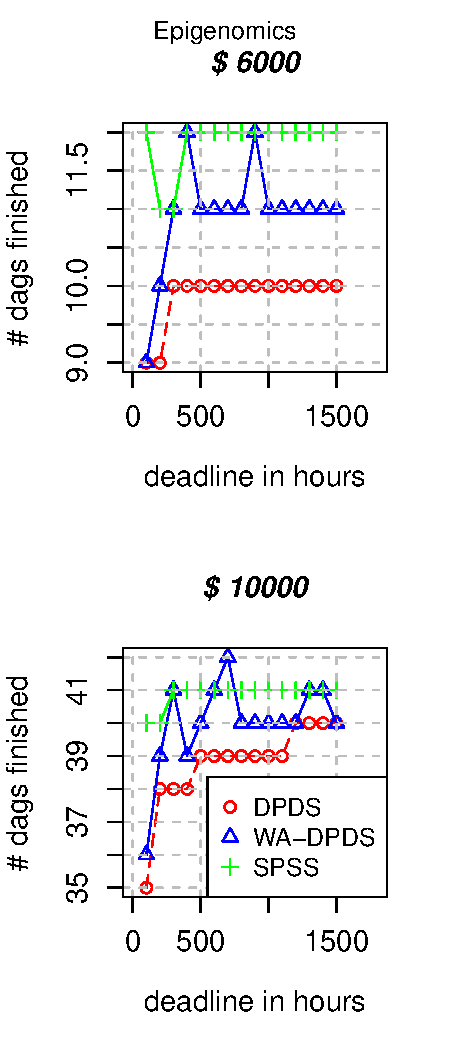
\includegraphics[width=0.19\textwidth]{figures/pareto-GENOME-n-1000-8-dagh100-1500m0.pdf}
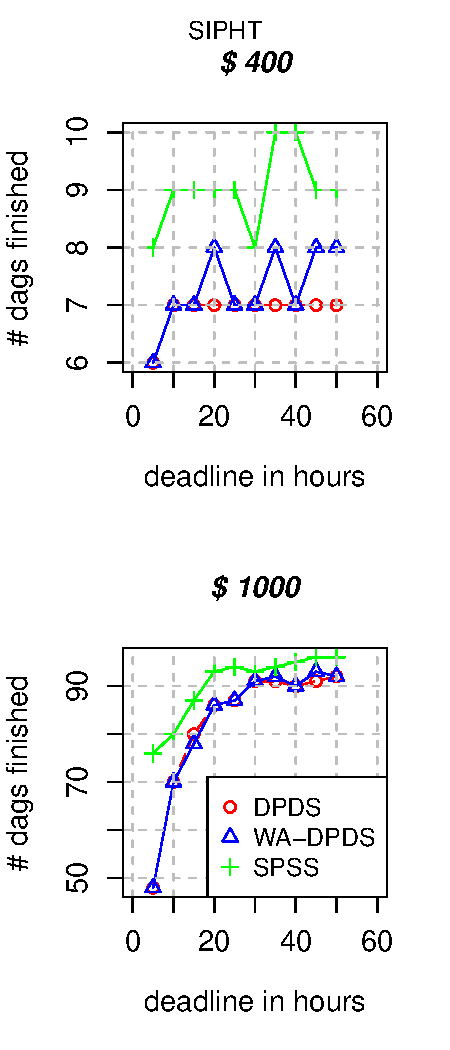
\includegraphics[width=0.19\textwidth]{figures/pareto-SIPHT-n-1000-8-dagh5-50m0.pdf}
\caption{Number of workflows completed for DPDS, AW-DPDS and SPSS
algorithms on ensembles of 100 Pareto-distributed workflows, {\em small budget}
(top) and {\em large budget} (bottom).}
\label{fig:number-complete-pareto}
\end{figure*}


%\begin{figure}[b!] 
%\centering
%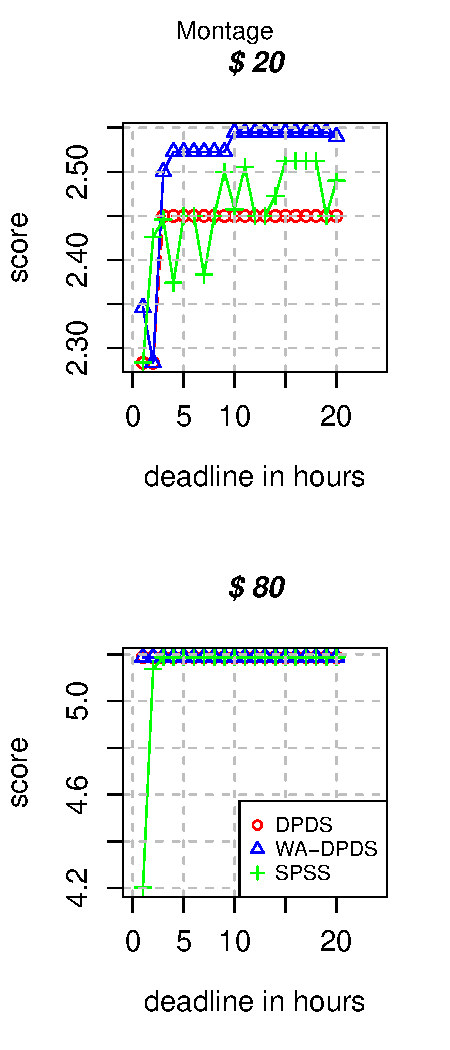
\includegraphics[width=0.19\textwidth]{figures/pareto-score-MONTAGE-n-1000-8-dagh1-20m0.pdf}
%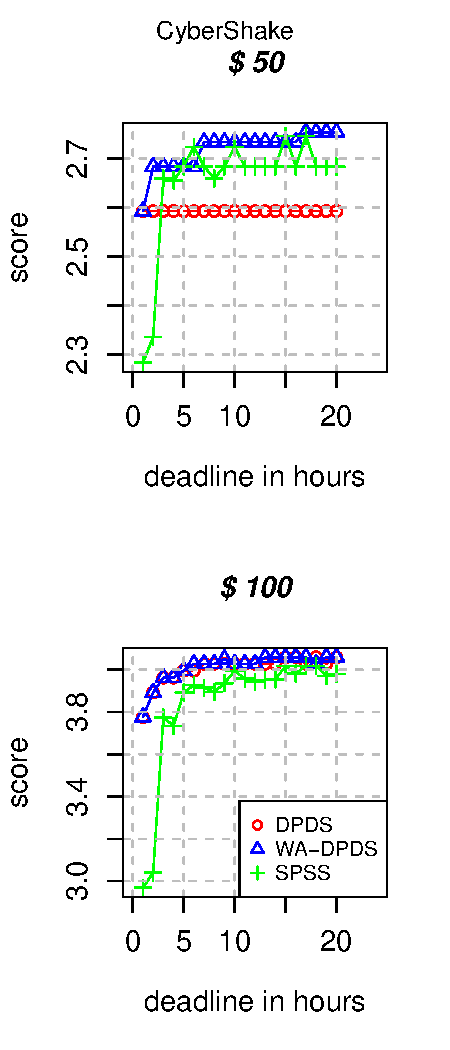
\includegraphics[width=0.19\textwidth]{figures/pareto-score-CYBERSHAKE-n-1000-8-dagh1-20m0.pdf}
%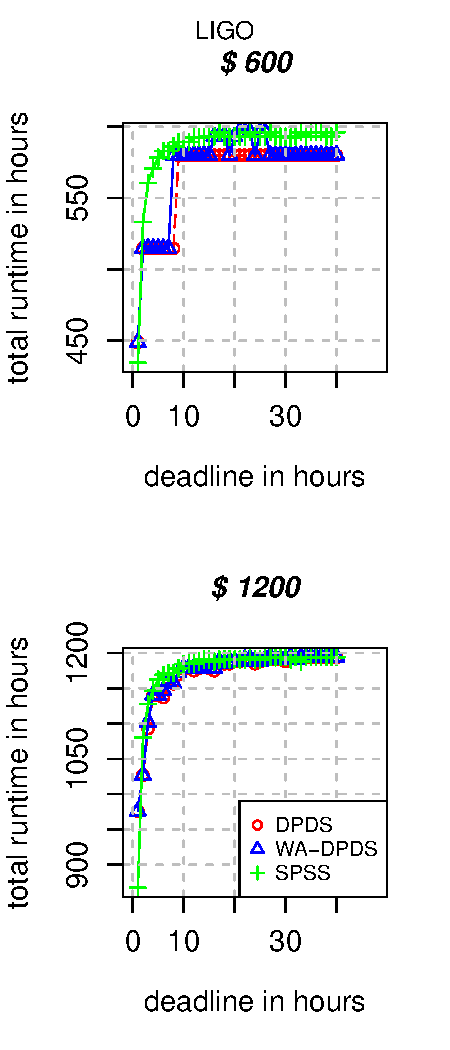
\includegraphics[width=0.19\textwidth]{figures/pareto-score-LIGO-n-1000-8-dagh1-40m0.pdf}
%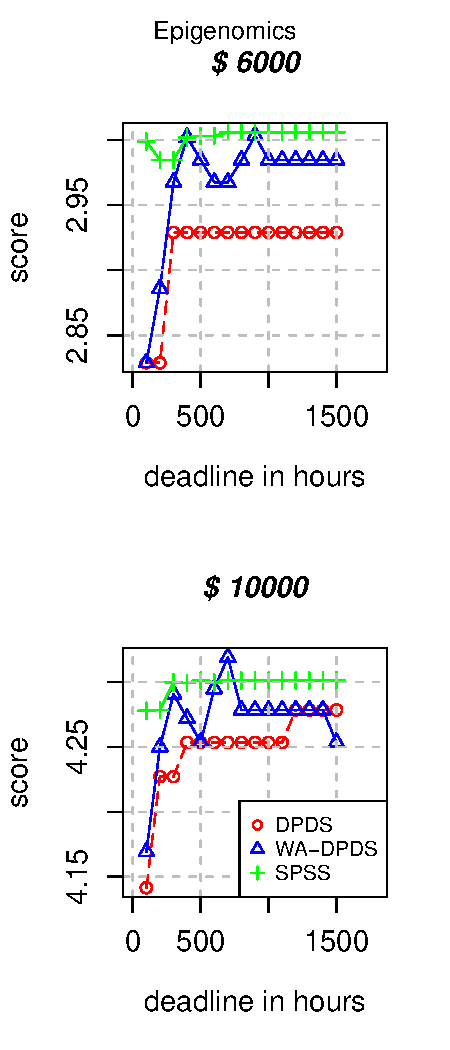
\includegraphics[width=0.19\textwidth]{figures/pareto-score-GENOME-n-1000-8-dagh100-1500m0.pdf}
%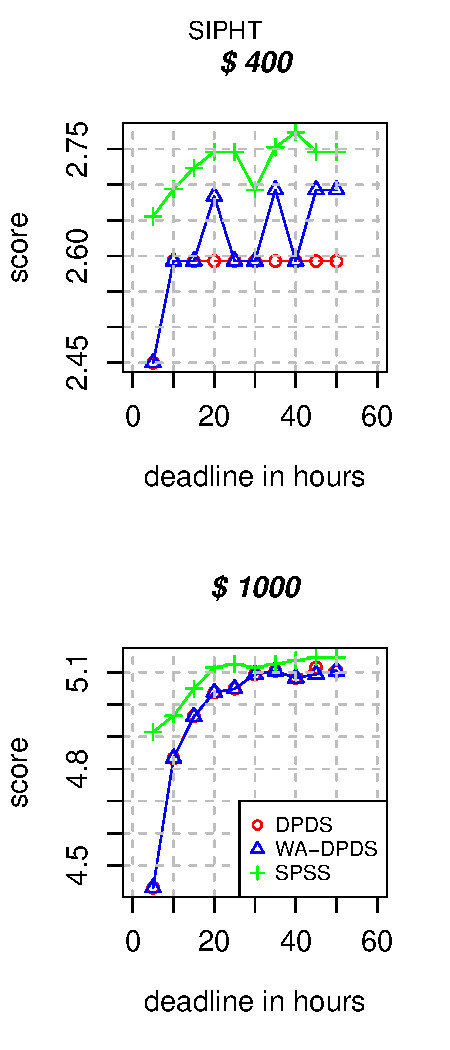
\includegraphics[width=0.19\textwidth]{figures/pareto-score-SIPHT-n-1000-8-dagh5-50m0.pdf}
%\caption{Comparison of algorithms based on score, which  is computed as
%$\sum(1/(p+1))$ where priorities of subsequent workflows are $p=0,1,2,\ldots$
%(0 means highest priority).}
%\label{fig:score}
%\end{figure}




In order to evaluate the algorithms on a standard set of workflows, we used
ensembles constructed from the DAGs available\footnote{\url{https://confluence.pegasus.isi.edu/display/pegasus/WorkflowGenerator}}
in the workflow generator gallery~\cite{Bharathi08}. The gallery contains
workflows of five applications from Pegasus as well as several other applications 
from~\cite{Ramakrishnan08}. We constructed ensembles of 100 DAGs by sampling the
workflows of different sizes based on a given distribution. By the size of the
workflow means the number of jobs. Two distributions are considered:
\begin{itemize}
  \item ensemble of workflows of equal size (constant)
  \item Pareto-like distribution.
\end{itemize}

Pareto-like distribution gives a small number of workflows with large size and a
large number of workflows with small size, as seen in
Fig.~\ref{fig:ensemble-distribution}. The number of largest
workflows (of size $\geq$ 900) is slightly increased to represent the
``long-tail'', i.e. that there is a non-insignificant number of large workflows
in the ensemble. The workflows are sorted according to their size and the largest workflows are
given the highest priority. 




\begin{figure*}[t]  
\centering
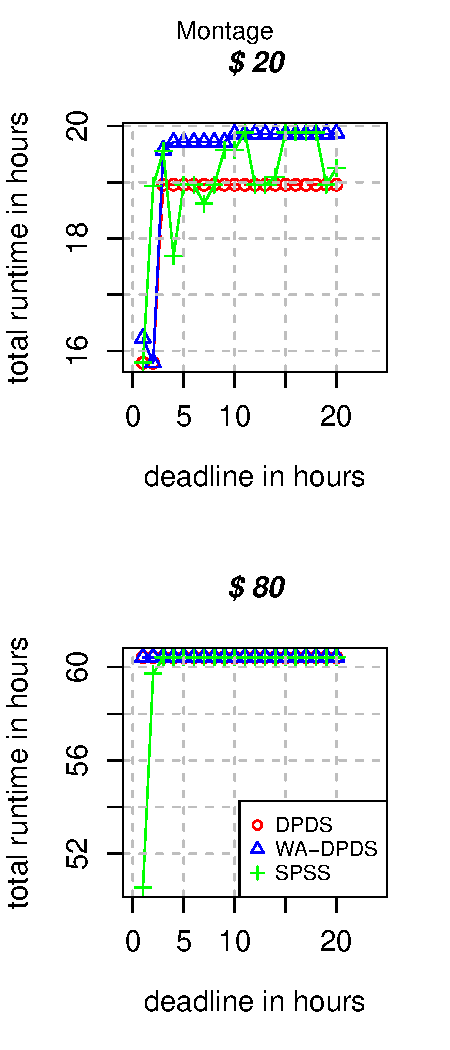
\includegraphics[width=0.19\textwidth]{figures/pareto-size-MONTAGE-n-1000-8-dagh1-20m0.pdf}
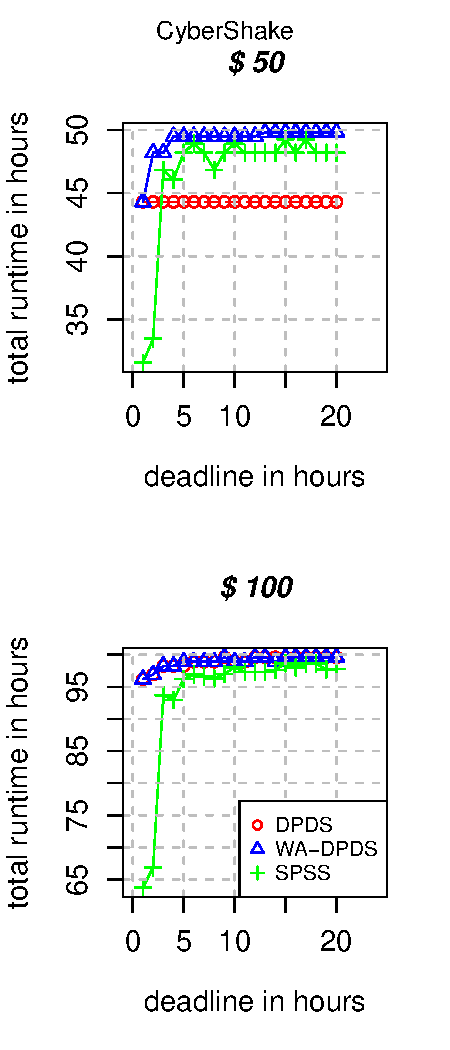
\includegraphics[width=0.19\textwidth]{figures/pareto-size-CYBERSHAKE-n-1000-8-dagh1-20m0.pdf}
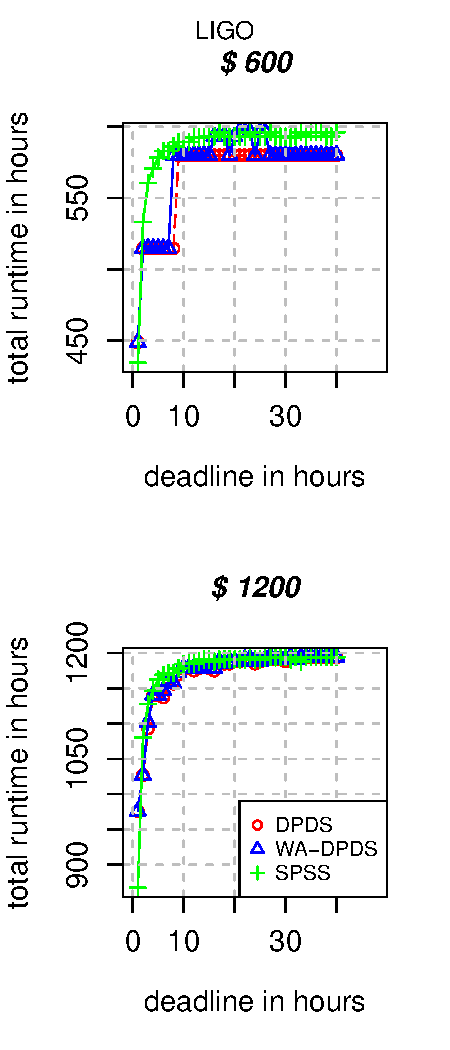
\includegraphics[width=0.19\textwidth]{figures/pareto-size-LIGO-n-1000-8-dagh1-40m0.pdf}
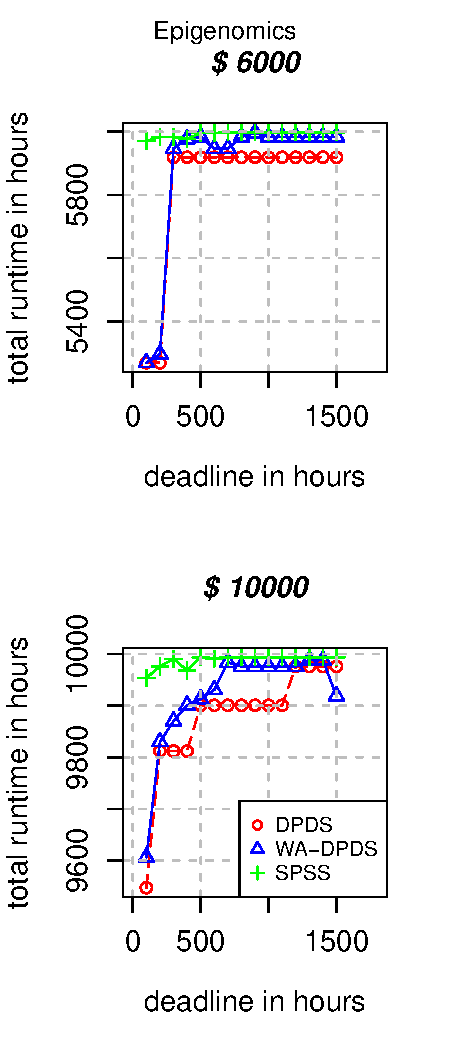
\includegraphics[width=0.19\textwidth]{figures/pareto-size-GENOME-n-1000-8-dagh100-1500m0.pdf}
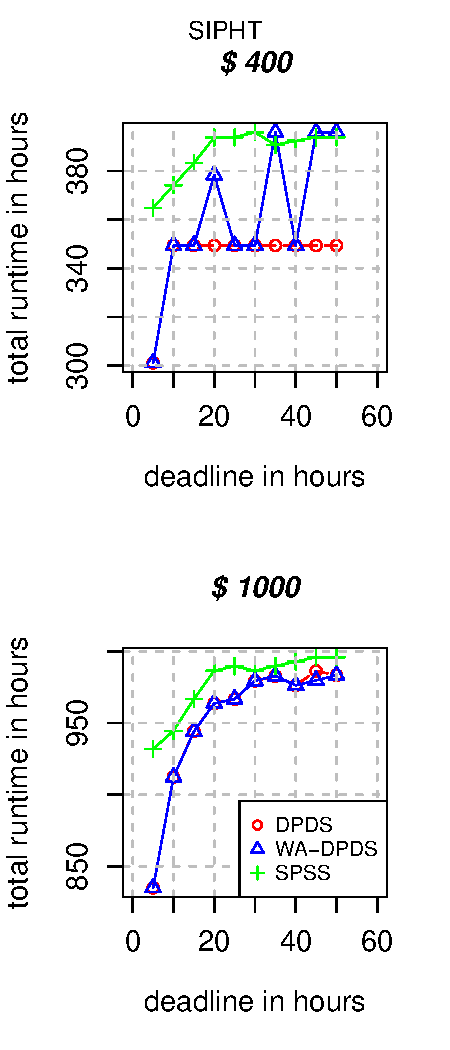
\includegraphics[width=0.19\textwidth]{figures/pareto-size-SIPHT-n-1000-8-dagh5-50m0.pdf}
\caption{ Total work completed expressed as the sum of runtimes (in hours) of
tasks of completed workflows. Data computed for DPDS, AW-DPDS and SPSS
algorithms on ensembles of 100 Pareto-distributed workflows}
\label{fig:total-time}
\end{figure*}


In the tests we we assumed that all the VMs are homogeneous and have the
processing speed of 1000 MIPS (million instructions per second), the price for
one VM-hour is \$1 and that the sizes of tasks in the workflow gallery are given
in seconds measured on 1000 MIPS machines. In this study we do not take into
account the heterogeneity of the infrastructure since we assume that it is
always possible to select a VM type that has the best price to performance ratio
for a given application.

For each application type, we selected such ranges of constraints (deadline,
budget) that it is possible to observe the possibly broad result space: from the
tight constraints, when only a small number of workflows can finish to the
liberal constraints when all or almost all the workflows can finish. These
parameters vary among the applications. Montage and CyberShake benchmarks
workflows required the budget in \$20 -- \$150 range and deadlines from 1 to
20 hours to complete the ensemble. LIGO and SIPHT workflows have more long
tasks, so they require budgets up to \$1,500 and deadlines extended to 40
hours. The Epigenomics workflow is even more costly and needs approximately \$12,000
and 1500 hours to complete the full ensemble.

We show the results for three algorithms: DPDS, WA-DPDS and
SPSS. These tests were run with maximum autoscaling factor set to 1.0 for
DPDS and WA-DPDS. After experimenting with DPDS and WA-DPDS we found that due to
high parallelism of workflows the resource utilization remains high most of the time, 
which leads to rapid provisioning of new resources at the beginning of ensemble
execution. This in turn results in less efficient total utilization due to high
level of parallelism. Setting the scaling limit to 1.0, ensures that the shape
of resource provisioning plan is closest to a rectangle (see
Fig.~\ref{fig:spds-example}) and the VM termination procedure
(Algorithm~\ref{alg:prov}) allows maximum utilization of VMs before shutdown.




\subsection{Metrics}




There are multiple ways to evaluate the algorithms and also different metrics
are relevant to the application users that are needed to take the planning
decisions. The set of metrics for each ensemble run we prepared includes:
\begin{itemize}
  \item number of workflows completed $N_c$,
  \item user preference score (utility function) $s$,
  \item total amount of computing time completed $T_C$,
  \item effective cost of computing per hour $C_{eff}$, which includes
  overheads.
\end{itemize}


The number of workflows completed is a simplest metric and allows distinguishing
which algorithm performs better. However, as the workflows have
different priorities and sizes, a less efficient algorithm may schedule smaller
low-priority workflows first, thus increasing the total number of workflows
complete. It may also happen that too conservative admission algoritm may reject
overestimate the costs of some large workflows, thus rejest some high-priority
ones which actually could fit into the schedule. Therefore we defined a user
preference score as:

%\begin{equation}
%\label{eq:score}
%s = \sum_{DAGs\ completed}(1/(p+1))
%\end{equation}


\begin{equation}
\label{eq:score}
s = \sum_{DAGs\ completed}2^{-p}
\end{equation}


where priorities of subsequent workflows in the ensemble are $p=0,1,2,\ldots$ (0
means highest priority). This exponential scoring function gives a strong weight
to the top priority workflows, since it has a property that a score for
completing a single workflow with priority $p$ is higher that the score for
completing all lower priority ones: 
\begin{equation}
\label{eq:score-property}
2^{-p} > \sum_{i=p+1,\ldots}2^{-i}
\end{equation}

Another metric is the total actual computing time completed and it is calculated
as the sum of all the runtimes of all the tasks of completed workflows. As in
our study we assumed that the resource cost pre hour is equal to \$1, the total
computing time can be easily compared to the allocated budget $b$. Their ratio
$u = (T_C * \$1)/b$ is the resource utilization and its inverse is the effective
resource cost: $C_{eff} = b/T_C$ in dollars per hour.

\subsection{Discussion of Results}




We run the simulations for the constraint values ranging between the
estimated limits as indicated in Section~\ref{sec:scenarios}, resulting in
ca. 50-150 (budget, deadline) points for each application. The runs were
repeated for Pareto-distributed and costant workflow sizes. From this result
space we selected the most interesting plots which give the good overview  of
the observed algorithm behavior.





\begin{figure*}[htb] 
\centering
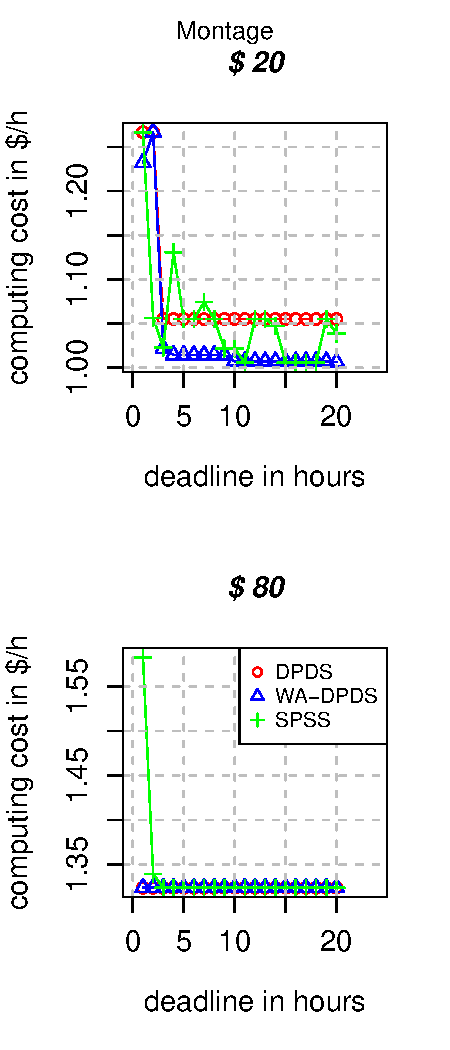
\includegraphics[width=0.19\textwidth]{figures/pareto-cost-MONTAGE-n-1000-8-dagh1-20m0.pdf}
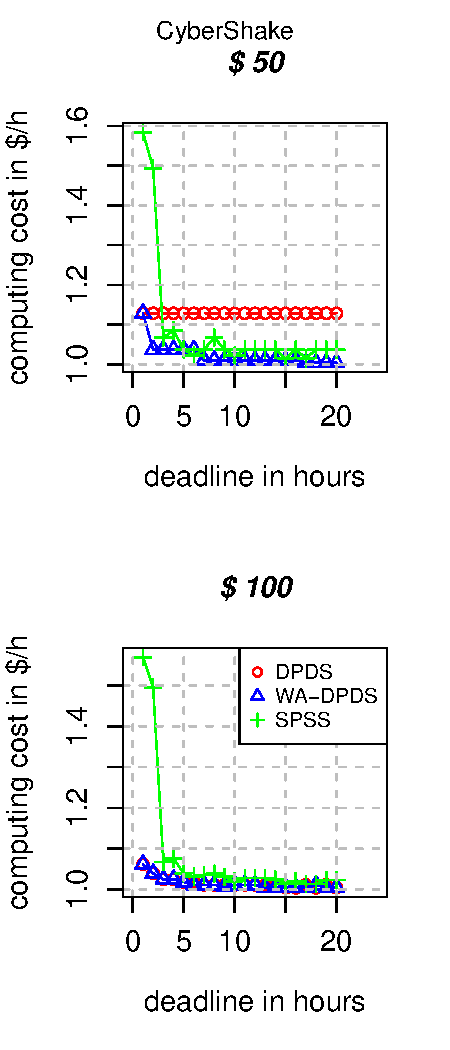
\includegraphics[width=0.19\textwidth]{figures/pareto-cost-CYBERSHAKE-n-1000-8-dagh1-20m0.pdf}
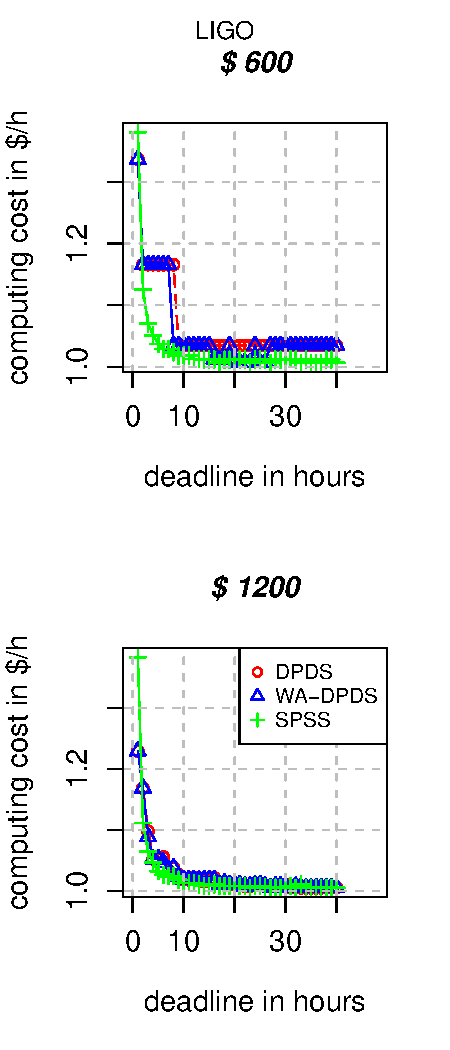
\includegraphics[width=0.19\textwidth]{figures/pareto-cost-LIGO-n-1000-8-dagh1-40m0.pdf}
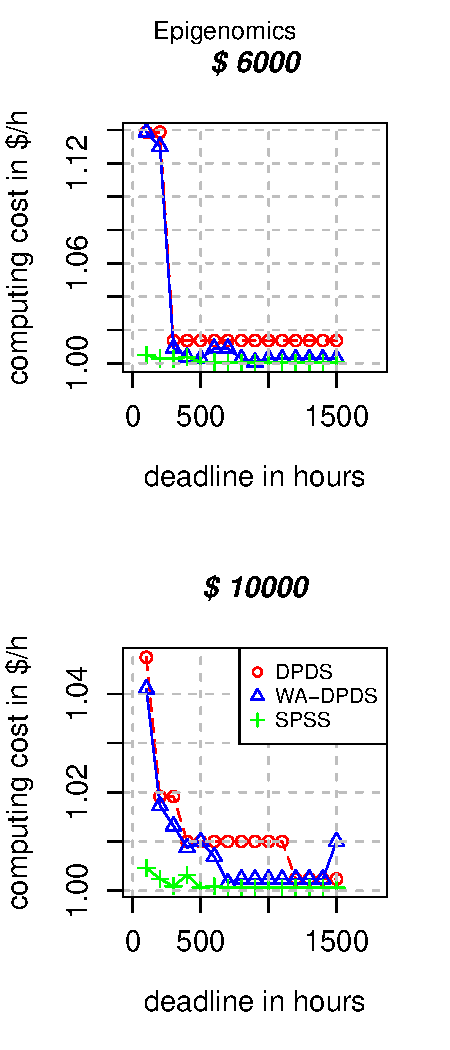
\includegraphics[width=0.19\textwidth]{figures/pareto-cost-GENOME-n-1000-8-dagh100-1500m0.pdf}
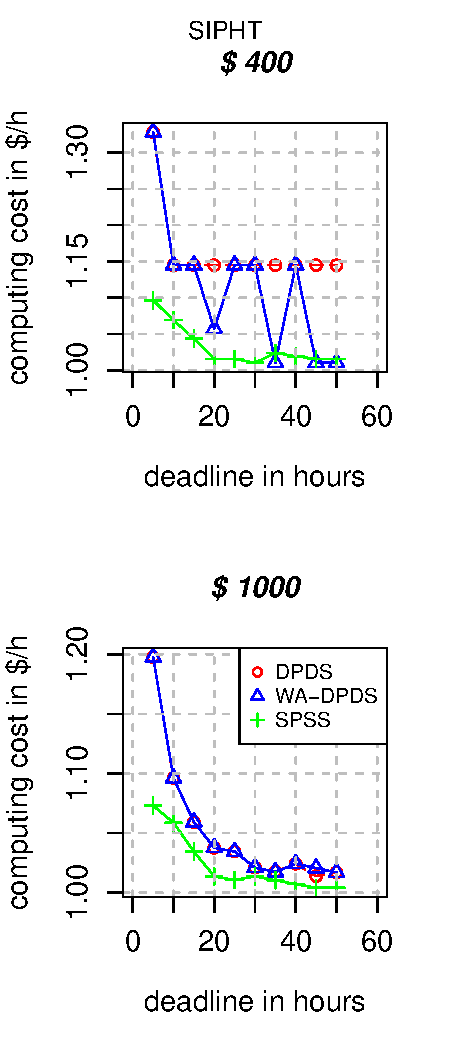
\includegraphics[width=0.19\textwidth]{figures/pareto-cost-SIPHT-n-1000-8-dagh5-50m0.pdf}
\caption{Effective computing cost in \$ per hour calculated by dividing sum of
task runtimes by the total budget. Higher cost results from lower resource utilization. Data based on DPDS, AW-DPDS and SPSS algorithms for ensembles of 100
Pareto-distributed workflows.}
\label{fig:cost}
\end{figure*}



Fig.~\ref{fig:number-complete-pareto} shows the number of the workflows
completed for two budget values per each application ensemble. The budget values
selected correspond to two opposite cases: {\em small budget} (top) and {\em
large budget} (bottom). The first one allows completing only a small number of
workflows from the ensemble, while the latter one suffices to finish almost all
the workflows. It can be seen that the static planning algorithm (SPSS) performs
better for tighter constraints: when the budget is low to admit only a small
number of workflows, the static procedure is able to more efficiently pack these
workflow tasks onto the resources. This can be clearly seen for the LIGO,
Epigenomics and SIPHT ensembles for small budgets and also for the same
ensembles with large budgets but short deadlines. The exception are Montage and
CyberShake ensembles, which consist of many fine-grained tasks that can be
executed in parallel. For these cases, as well for the other ensembles with
large budgets, the simple dynamic scheduling techniques perform equally well or
better. The reason for that behavior is that the large number of tasks
guarantees that resources are almost never idle, while the provisioner algorithm
makes sure that the VM instances are most efficiently utilized before shutdown.
We can also observe that the workflow-aware dynamic algorithm (WA-DPDS) performs
better than the workflow-unaware version. This means that for the tested
workflows the simple admission procedure based on estimation of workflow cost
does not degrade the solution, but rather in many cases it allows rejecting
larger workflows that would lead to budget overrun. Thus it can save the space
for smaller workflows that can complete.





%Fig.~\ref{fig:score} shows the score $s$ as defined in Eq.~\ref{eq:score}
%computed for two sample applications. Comparing
%Fig.~\ref{fig:number-complete-pareto} to Fig.~\ref{fig:score} we can see that
%the latter one gives more flattened shape: this means that e.g. the improvement
%of the solution by one workflow may mean adding a one low-priority workflow.
%Nevertheless we can see that the curves on both figures have a very similar
%shape, which mens that our algorithms obey the priority rules and do not try to
%admit lower-priority workflows at the cost of the more important ones.

\begin{figure}[htb] 
\centering
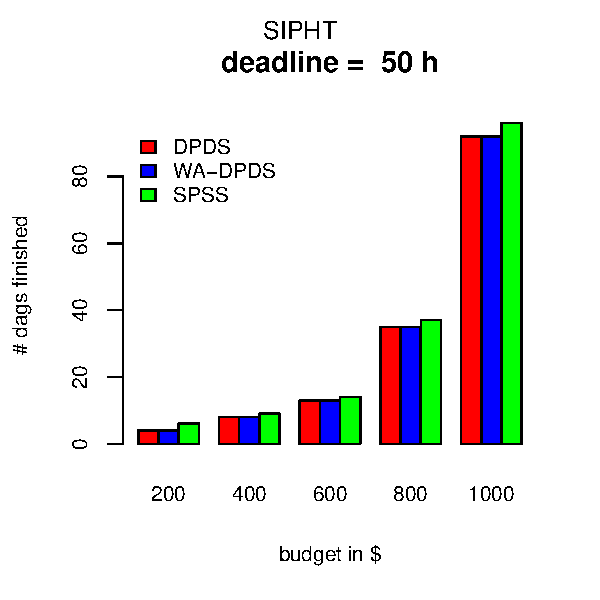
\includegraphics[width=0.6\columnwidth]{figures/pareto-budget-SIPHT-n-1000-8-dagh5-50h10m0.pdf}
\caption{Comparison of number of workflows completed for a given deadline,
plotted versus different budget amounts.}
\label{fig:budgets}
\end{figure}



\begin{table}[tb]
\centering

(a) Number of workflows completed $N_c$:
\medskip
\begin{tabular}{r|cccccc}
 & M & C & L & E & S & All\tabularnewline
\hline
DPDS      &   57  & 45 &  18 &  14  &  0 & 134\tabularnewline
WA-DPDS   &    96 &  87  & 48  & 34  &  0 & 265\tabularnewline
SPSS     &    29  & 42  & 192  & 74  & 50 & 387\tabularnewline
\end{tabular}
\medskip

(b) Total amount of computing time completed $T_C$:
\medskip
\begin{tabular}{r|cccccc}
 & M & C & L & E & S & All\tabularnewline
\hline
DPDS      &   58  & 45 &  19 &  14  &  0 & 136\tabularnewline
WA-DPDS   &    90  & 96  & 57  & 27 &   8 & 278\tabularnewline
SPSS     &    31 &  18 &  170  & 75 &  42 & 336\tabularnewline
\end{tabular}
\medskip

(c) Exponential score $s$:
\medskip
\begin{tabular}{r|cccccc}
 & M & C & L & E & S & All\tabularnewline
\hline
DPDS      &   58  & 45 &  19 &  14  &  0 & 136\tabularnewline
WA-DPDS   &    90  & 96  & 57  & 27 &   8 & 278\tabularnewline
SPSS     &    31 &  18 &  170  & 75 &  42 & 336\tabularnewline
\end{tabular}
\medskip

\label{tab:num-dags-pareto}
\caption{Number of times each algorithm achieved the highest score 
over all budgets and deadlines. Data from a total of 525 runs on 
Pareto-distributed ensembles for Montage (M), CyberShake (C), LIGO (L), 
Epigenomics (E), SIPHT (S).}
\end{table}


Fig.~\ref{fig:total-time} presents the same results using the total computing
time metric $T_C$. These plots confirm our previous observations about the
algorithms performance, but they also allow to observe a more general property.
For a given budget, when the deadline is tightened the number of work done
steeply decreases. Assiging a shorter deadline means that more VMs need to be
provisioned to complete the work, but this leads to higher parallelism and thus
to the lower parallel efficiency. E.g. running 2 VMs for 10 hours will be more
efficient than running 10 VMs for 2 hours. Therefore, if deadline permits and
costs are important, parallelism should be avoided when possible.

These observations are further confirmed when examining the efffective resource
cost, as shown in Fig.~\ref{fig:cost}. It can be seen that lower resource
utilization and lower parallel efficiency for short deadlines lead to
substantial increase of actual costs of computing. This increase reaches
$\sim$20\%, which means that if we need to run e.g. a SIPHT workflow ensemble
with a short deadline, $\sim$\$200 out of \$1000 is spent on idle resources.

Another general conclusion can be drawn from Fig.~\ref{fig:cost}: despite some
random fluctuations resulting mostly from the finite result space, all the
curves for all the applications and budgets have a similar shape. This shape
represents a trade-off curve between two conflicting objectives: time and cost.
We can see that the selection of deadline and cost can be formulated as
multi-criteria optimization problem and the curves presented in
Fig.~\ref{fig:cost} are approximations of the Pareto front (or Pareto set) of
solutions to this problem. In our case the solutions were achieved by maximizing
the number of work done, which direcly results in minimization of effective cost parameter for a given
deadline. Therefore, the obtained results can be used to assist the decison in
resource allocation planning, when both cost and time criteria are given not as
constraints but as objectives.


% \begin{figure*}[htb] \centering
% 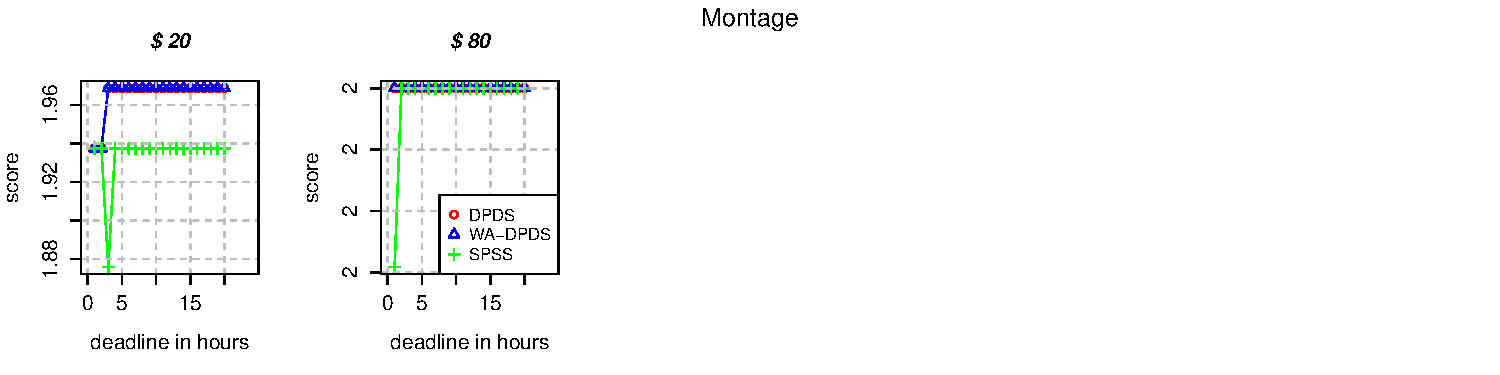
\includegraphics[width=0.19\textwidth]{figures/score2-MONTAGE-n-1000-8-dagh1-20m0.pdf}
% 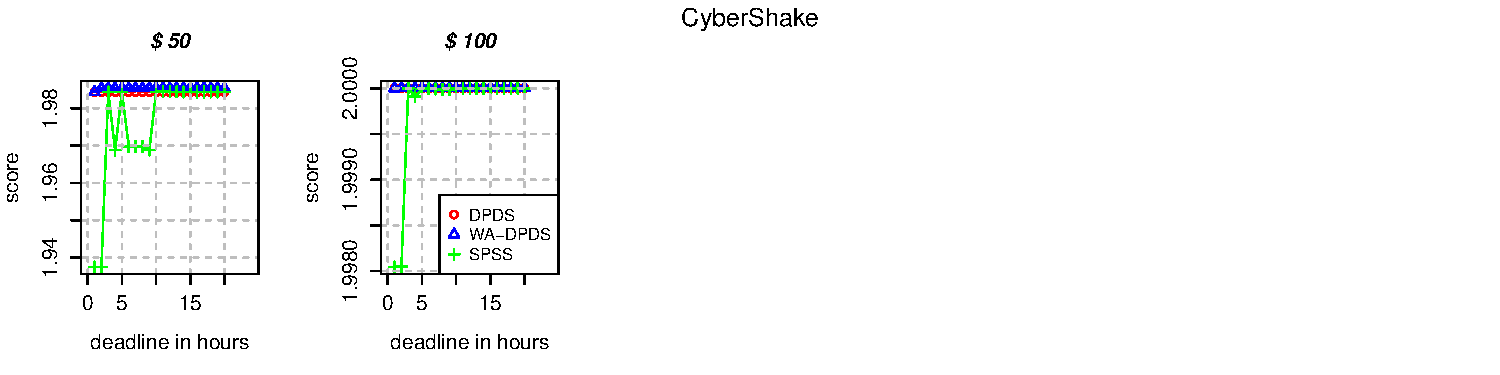
\includegraphics[width=0.19\textwidth]{figures/score2-CYBERSHAKE-n-1000-8-dagh1-20m0.pdf}
% 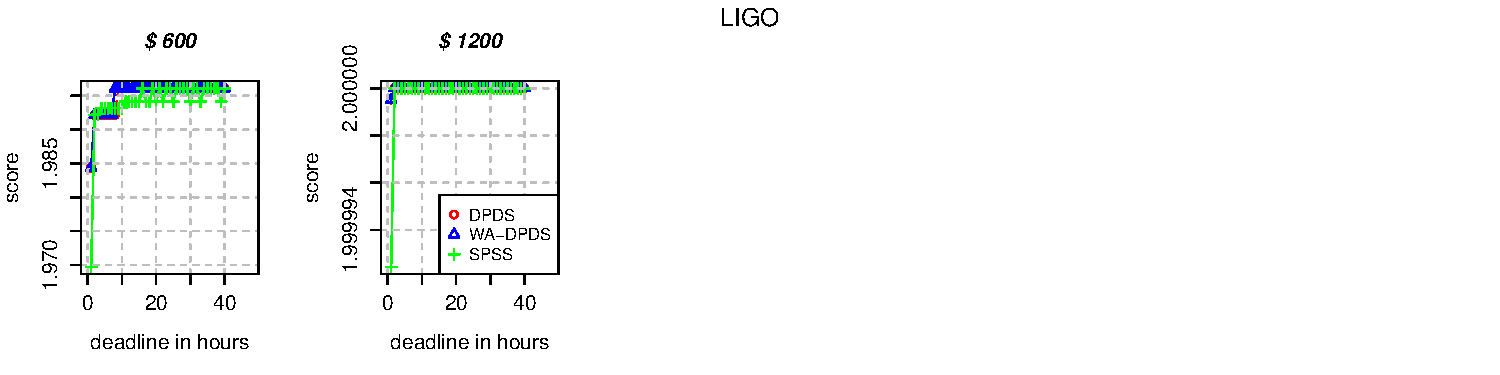
\includegraphics[width=0.19\textwidth]{figures/score2-LIGO-n-1000-8-dagh1-40m0.pdf}
% 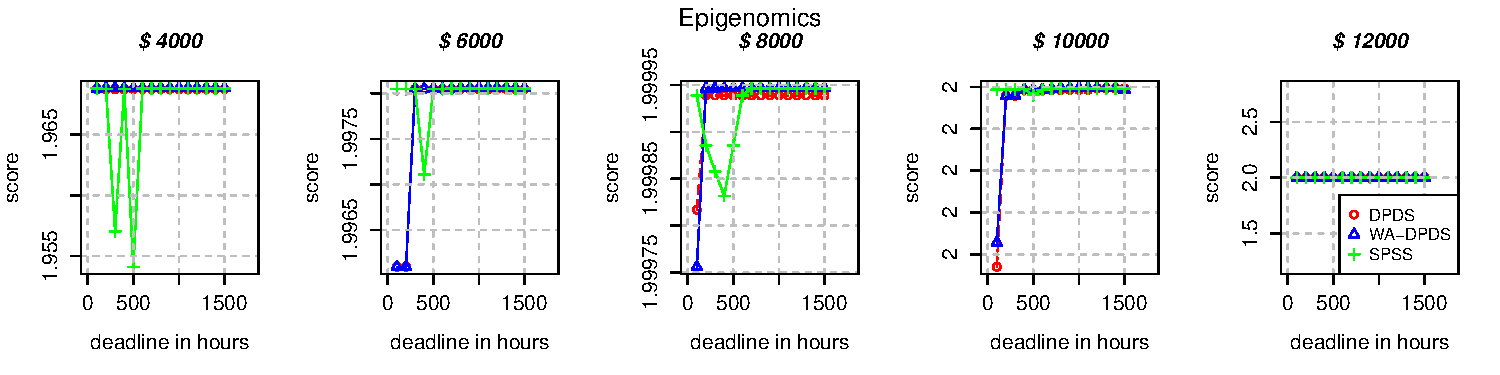
\includegraphics[width=0.19\textwidth]{figures/score2-GENOME-n-1000-8-dagh100-1500m0.pdf}
% 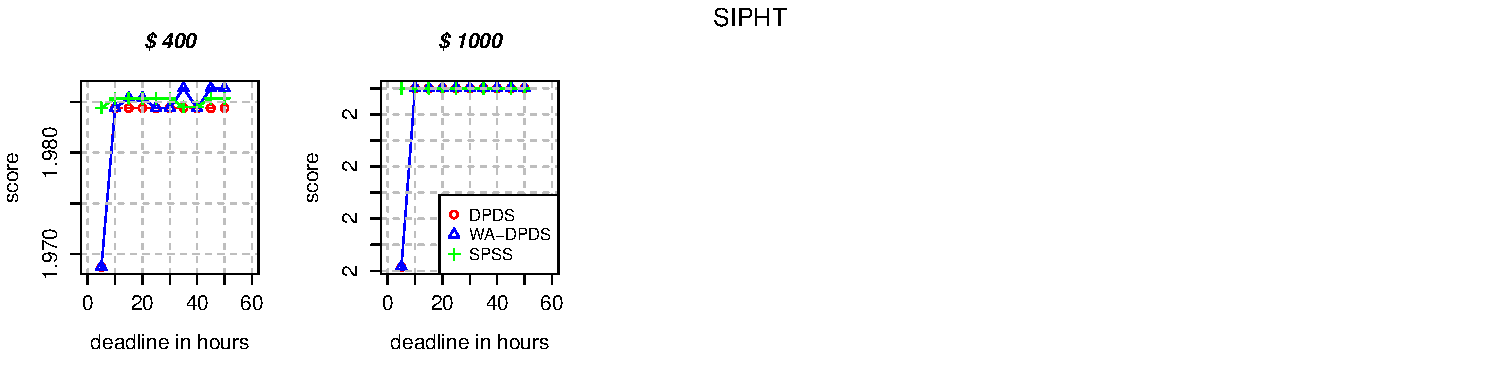
\includegraphics[width=0.19\textwidth]{figures/score2-SIPHT-n-1000-8-dagh5-50m0.pdf}
% \caption{Comparison of DPDS, AW-DPDS and SPSS algorithms for ensembles of 100
% Pareto-distributed workflows. Score is computed as $\sum(2^(-p))$ where
% priorities of subsequent workflows are $p=0,1,2,\ldots$ (0 means highest
% priority).} \label{fig:} \end{figure*}
       
               
In order to compare efficiency of algorithms, we counted the number of times
each algorithm achieved the best results for all tested applications, deadlines
and budgets. If two or more algorithms achieve the same highest results, all are
counted as highest. Table~\ref{tab:num-dags-pareto} shows these summary values.
These results depend on the metric: number of workflows completed does not count
the priorities or sizes of workflows, which means that it happens more often
that all the algorithms achieve the same (best) result. However, it does not
mean that all algorithms complete the same workflows: that is why values
in the tables (a), (b) and (c) are different. it can be observed that based on
the sampled problem space the workflow-aware algorithms achieve highest score
in $\sim$2--3 times more cases than the simple DPDS which does not take into
account workflow structure or size. In average, SPSS performs better in
$\sim$20--50\% more times than WA-DPDS. We have to note, that the sampled
paramter space included the Montage and CyberShake workflows consisting of many
small tasks, for which cases SPSS does not perform equally well. 
               
               
Fig.~\ref{fig:budgets} whows the same data for SIPHT ensemble from another
perspective. It helps answer the question: given a deadline, how many workflows
can be finished when we increse the budget. In Fig.~\ref{fig:budgets} the growth
is super-linear, what results from the distribution of workflow sizes in the
ensemble (see Fig.~\ref{fig:ensemble-distribution}). For ensemble of equal size
workflows (see Fig. TODO: ADD FIGURE FROM CONSTANT DISTRIBUTION) the growth is
nearly linear. It can be also observed that staitc algorithms give better
results for smaller budgets, while dynamic algorithms for larger ones.




\section{Conclusion and Future Work}

In this paper we addressed a new interesting and important problem of scheduling
and resource provisioning for scientific workflow ensembles on IaaS cloud
infrastructures. The problem is different from previous work on grid or utility
grid scheduling that cloud infrastructure gives more control over the resources,
so the resource provisioning plan can be adjusted to the application
requirements. Therefore the problem space becomes larger: it requires not
only to select the best scheduling of tasks to available resources, but also
select the best shape of resource provisioning plan. The formulation of a
problem as maximization of the number of prioritized workflows completed from
the ensemble requires also to take the decisions on admitting or rejecting workflows
based on their estimated resource demands. We believe that such formulation of
the bi-constrained problem is highly relevant since such
constraints are typically imposed on many real-world projects.

We have analyzed both static and dynamic scheduling approaches and
developed the SPDS, DPDS, WA-DPDS and SPSS algorithms realizing these
strategies. The algorithms were evaluated on ensembles of benchmark
workflows which represent typical real scientific applications. For the
purpose of evaluation we have developed a simulator that models the cloud
infrastructure and the tightly-coupled scheduler and provisioner modules of
workflow engine. The results of simulation studies indicate that the two algorithms (WA-DPDS and
SPSD) that take into account the information about the workflow structure and
estimation of task runtimes yield better results than the simple on-line
priority-based scheduling strategy with static (constant) resource provisioning
plan. 

During our work, several interesting lessons were learned about the workflow
ensembles on cloud infrastructures. One result is that the simple strategy of
SPDS performs relatively well in terms of number of workflows completed and the
high resource utilization it can achieve. However, this method does not allow to
give any advance prediction about the result, so to see its performance the
whole ensemble needs to be simulated. On the other hand, the method may be
the only choice in the case no estimates about the task runtimes are available
in advance. It can be seen that the workflow-aware and static algorithms are
able to find better quality solutions in terms of the defined metrics: this the
result mainly of the admission algorithm implemented, which allow rejecting too
large workflows and thus saving resources for completing the less costly ones.

Another general observation is that although clouds provide such capabilities as
dynamic adding and removing of resources at runtime and high parallelization due
to ilusion of unlimited resources, it turns out that is recommended to avoid
using these capabilities when possible, in order to achieve high resource
utilization and cost effectiveness. This observation comes from the fact that
starting and stopping more VMs incurres a cost which can be amortized by running
each started VM as long as possible before shutdown. This effect was confirmed
in the case of SPSS algorithm for Montage and CyberShake workflows with small
budgets. Similarly, high degree of parallelization (large number of nodes) leads
also to less efficient resource utilization and in the case of clouds the drop
in parallel efficiency means also the increase of cost. This result, clearly
visible in Fig~\ref{fig:cost}, leads to multi-criteria decision problems and
related trade-offs. E.g. our simulation results can be used as hints to answer
the question how much time and money is required to actually complete all the
workflows from the given ansemble.

Another lesson learned from our studies is related to the shapes and granularity
of the tasks of workflows in the ensembles. The benchmarks workflows that we
tested have relatively large number of tasks (50--1000). Montage and CyberShake
workflows have fine-grained tasks of short execution times, in the order of
seconds and minutes. LIGO, Epigenomics and SIPHT have longer tasks: from minutes to hours.
Therefore the dynamic algorithms achieved better results on the fine grained
workflows, since the simple random-based allocation strategy leads to good
load-balancing and high resource utilization. On the other hand, when tasks are
longer, it becomes more beneficial to apply a static planning strategy of SPSS.

Our current study reveals multiple paths for future work. One interesting
question would be to answer how the static and dynamic algorithms perform in the
cases of increased uncertainities and failures, that have important influence
on overall system performance~\cite{Sakellariou2010,Dongarra2007}. Second
important goal would be to extend our application and infrastructure model to
include various data storage options available on clouds. The experimental study
on that subject~\cite{Juve2010} suggests that data demands of scientific
workflows have a high impact not only on execution time but also on costs on
commercial clouds. Finally, we would like to address the heterogeneity of the
infrastructure, as multiple instance types and providers, including private
and community clouds will make the problem more complex and
challenging~\cite{Marshall2010,vockler11,Juve2010}.


%\section{Acknowledgments}
%Acknowledgements go here.

\bibliographystyle{abbrv}
\bibliography{paper}

%\appendix
%\section{Headings in Appendices}

%\balancecolumns

\end{document}
